
\documentclass[../main.tex]{subfiles}
\begin{document}
    \section{I/O Avoiding Algorithms}
	\begin{mdframed}[style=Quiz]
		\textbf{Given:}
		\begin{itemize}
			\item Volume of data to sort $\equiv r \cdot n = 1 PiB (=2^{50})$ Bytes
			\item Record (item) size $\equiv r = 256$ Bytes
			\item Fast memory size $\equiv r \cdot z = 64 GiB (=2^{36}B)$
			\item Memory transfer size $\equiv r \cdot L = 32 KiB (=2^{15}B)$
		\end{itemize}
		
		\noindent
		\textbf{Question:} What is the performance of various equations?
		
		\noindent
		\textbf{Answer:}
		\begin{center}
			
			\begin{tabular}{cccccc}
				$n\log_2n$ & $n\log_2\frac{n}{L}$ & $n$ & $\frac{n}{L}\log_2\frac{n}{L}$ &$\frac{n}{L}\log_2\frac{n}{Z}$ &$\frac{n}{L}\log_{\frac{Z}{L}}\frac{n}{Z}$\\
				\hline
				185& 154& 4.40& 1.20 &0.275& 0.0523 \\
			\end{tabular}
		\end{center}
		
		\noindent
		\textbf{Note:} importantly the biggest improvement comes when going from $n\log_2$ to $\frac{n}{L}\log_2$ because we we iterate through the data, we do it in $L$ chunks vs one at a time. The other big improvement comes from going from $\log_2$ to $\log_{\frac{Z}{L}}$ This improvement involves the capacity of fast memory $Z$, this maximises useage of fast memory.
	\end{mdframed}
	\subsection{External Memory Mergesort} Imagine an array with n elements. How can we perform a merge sort on that algorithm? First we divide the array into blocks of $Z$ size.
	\begin{center}
		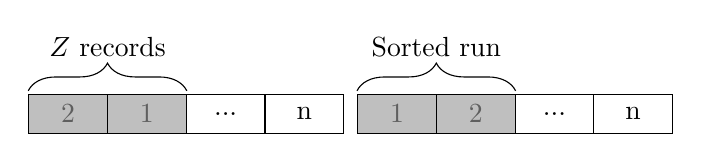
\begin{tikzpicture}
			\node[rectangle,
			draw,
			text = black
			, fill=gray
			,fill opacity=.5
			,minimum width = 1cm
			, minimum height =.5cm] (1) at (0,0) {2};
			\node[rectangle,
			draw,
			text = black
			, fill=gray
			,fill opacity=.5
			,minimum width = 1cm
			, minimum height =.5cm] (2) [right of=1] {1};
			\node[rectangle,
			draw,
			text = black
			,minimum width = 1cm
			, minimum height =.5cm] (...) [right of=2] {...};
			\node[rectangle,
			draw,
			text = black
			,minimum width = 1cm
			, minimum height =.5cm] (n) [right of=...] {n};
			\draw [decorate,
			decoration = {brace,raise=1pt,amplitude=10}] (1.north west) -- (2.north east)node[pos=0.5,above=10pt,black]{$Z$ records};
					\node[rectangle,
			draw,
			text = black
			, fill=gray
			,fill opacity=.5
			,minimum width = 1cm
			, minimum height =.5cm] (3) [xshift=5,right of=n] {1};
			\node[rectangle,
			draw,
			text = black
			, fill=gray
			,fill opacity=.5
			,minimum width = 1cm
			, minimum height =.5cm] (4) [right of=3] {2};
			\node[rectangle,
			draw,
			text = black
			,minimum width = 1cm
			, minimum height =.5cm] (...2) [right of=4] {...};
			\node[rectangle,
			draw,
			text = black
			,minimum width = 1cm
			, minimum height =.5cm] (n2) [right of=...2] {n};
			\draw [decorate,
			decoration = {brace,raise=1pt,amplitude=10}] (3.north west) -- (4.north east)node[pos=0.5,above=10pt,black]{Sorted run};
		\end{tikzpicture}
	\end{center}
We then load this chunk and sort it writing it back to the array producing a \textbf{(sorted) run}. repeat this process until all $\frac{n}{fZ}$ chunks are sorted runs. This is \textbf{Phase 1} of the procedure.
\begin{mdframed}[style=Quiz]
	\textbf{Question:} What are the total Asymptotic costs?
	
	\noindent
	\textbf{Answer:}
	\begin{enumerate}
		\item Read Chunk $o(\frac{n}{L})$
		\item comparisons $o(n\log z)$
		\item Read Chunk $o(\frac{n}{L})$
	\end{enumerate}
\end{mdframed}
\begin{center}
    \begin{tikzpicture}
        
    \end{tikzpicture}
\end{center}
\end{document}